\documentclass[letterpaper,10pt]{article}

%\setlength{\parindent}{0in}
%\usepackage{fullpage} 
\usepackage{amsmath}
\usepackage{enumerate}
\usepackage{graphicx}
\oddsidemargin 0.0in
\textwidth 6.5in

%opening
\title{Homework for Module 5}
\author{Steve Mazza}

\begin{document}
\maketitle

\begin{description}
\item[6.1.1]\ 
\begin{enumerate}[a)]
\item The population is defined by the set of all possible rolls of the dice.  $(X:x \mid x \in \{1, 2, 3, 4, 5, 6\})$
\item There are no additional factors that should be taken into account.  For fair dice, there are no issues pertaining to the way in which the sample has been controlled.
\end{enumerate}

\item[6.2.5]
%TODO: Insert an appropriate graphical representation of DS 6.1.1
There appear to be no outliers and the data set looks like I would expect it to.

\begin{center}
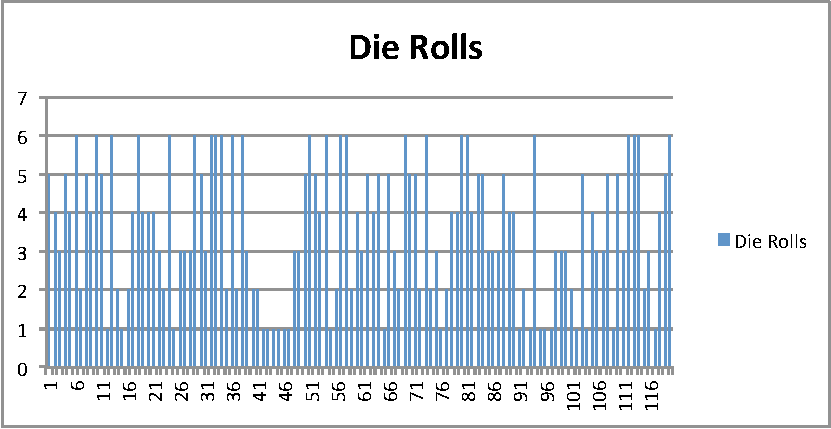
\includegraphics[scale=0.75]{module5b.pdf}
\end{center}

\begin{center}
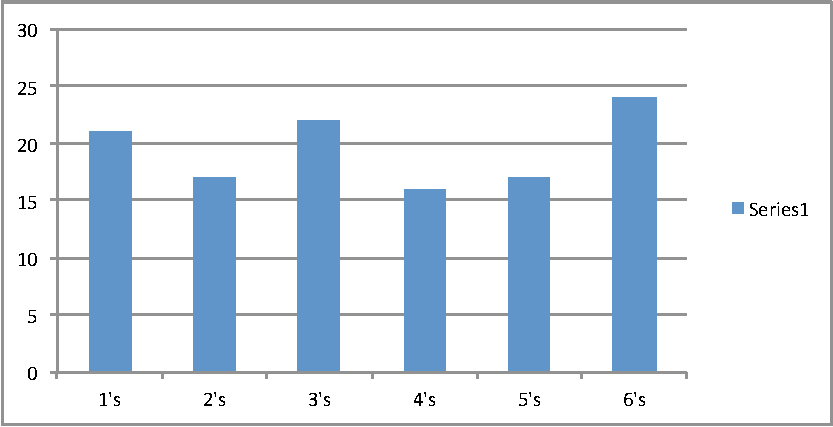
\includegraphics[scale=0.75]{module5c.pdf}
\end{center}

\item[6.3.4]
There appear to be no anomolies in the sample statistics.  The results are appropriate for the sample size.
\begin{table}[htdp]
\caption{Summary Statistics}
\begin{center}
\begin{tabular}{|c|c|}\hline
Mean & 3.567 \\
Standard Error & 0.161 \\
Median & 3.5 \\
Mode & 6 \\
Standard Deviation & 1.767 \\
Sample Variance & 3.122 \\
Kurtosis & -1.319 \\
Skewness & -0.033 \\
Range & 5 \\
Minimum & 1 \\
Maximum & 6 \\
Sum & 428 \\
Count & 120 \\
\hline
\end{tabular}
\end{center}
\label{default}
\end{table}

\begin{center}
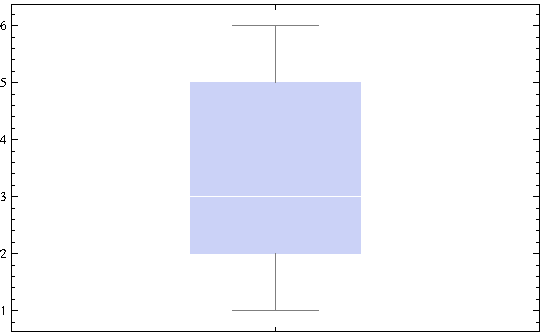
\includegraphics[scale=0.75]{module5a.pdf}
\end{center}


\item[7.2.9] %\theta \sigma
To find the standard deviation, $\sigma$, of $\frac{X_{1}+X_{2}}{2}$ first calculate $\mbox{Var}(\frac{X_{1}+X_{2}}{2})$.
\begin{align*}
\mbox{Var}\frac{X_{1}+X_{2}}{2} &= \frac{\mbox{Var}(x_{1}+\mbox{Var}(x_{2}}{4} \\
&= \frac{5.39^{2}+9.43^2}{4} \\
&\approx 29.49 \\
\sigma &= \sqrt{29.49} \\
&\approx 5.43
\end{align*}

\item[7.3.3]\  %\mu
\begin{enumerate}[a)]
\item \[P(\mid N(0,\frac{7}{15})\mid\leq 0.4) \approx 0.4418\]
\item \[P(\mid N(0,\frac{7}{50})\mid\leq 0.4) \approx 0.7150\]
\end{enumerate}

\item[7.3.7]
Applying the definition of $t$-statistic from page 311,
\begin{enumerate}[a)] 
\item \
\[P(\frac{\left| t_{21-1}\right|}{\sqrt{21}} \leq c) = 0.95\]
And now solving for $c$
\begin{align*}
c &= \frac{t_{0.025,20}}{\sqrt{21}} \\
&\approx 0.4552
\end{align*}
\item \ 
\[P(\frac{\left| t_{21-1}\right|}{\sqrt{21}} \leq c) = 0.99\]
And now solving for $c$
\begin{align*}
c &= \frac{t_{0.005,20}}{\sqrt{21}} \\
&\approx 0.6209
\end{align*}
\end{enumerate}

\item[7.3.10]\ 
\begin{enumerate}[a)]
\item Point estimate of the probability of rolling a 6:
\[\frac{24}{120} = 0.2\]
\item Standared error of point estimate:
\begin{align*}
\mbox{s.e.}\hat{p} &= \sqrt{\frac{\hat{p}1-\hat{p}}{n}} \\
&= \sqrt{\frac{0.2\times 0.8}{120}} \\
&\approx 0.036515
\end{align*}
\end{enumerate}

\item[7.6.12] %\Phi
Using sample size $n=80$ and $p=0.48$, given, calculate:
\[P(0.48-0.1\leq\hat{p}\leq0.48+0.1)\simeq P(80\times0.38\leq B(80,0.48)\leq 80\times 0.58)\]
Then apply the Normal approximation to $B(n,p)$ from page 240:
\begin{align*}
\Phi(\frac{46.4+0.5-80\times 0.48}{\sqrt{80\times 0.48\times 0.52}})-\Phi(\frac{30.4+0.5-80\times 0.48}{\sqrt{80\times 0.48\times 0.52}}) &= \\
&\approx \Phi(1.9022)-\Phi(-1.6784) \\
&\approx 0.9714-0.0466 \\
&\approx 0.9248
\end{align*}

\end {description}
\end{document}